\documentclass[xcolor=table,usenames,dvipsnames]{beamer}

\usepackage{lscape, amsmath, amsfonts, amssymb, setspace, theorem, wrapfig, graphicx, float, multirow, subfig, color, rotating, multicol, datetime, natbib, venndiagram, pstricks, xkeyval, tikz, etoolbox, url, hyperref, nth}

\usepackage[T1]{fontenc}
\usepackage[latin1]{inputenc}
\usepackage[english]{babel}
\usetikzlibrary{arrows,calc,matrix}

\title{GV217 - Conflict Analysis}
\subtitle{University of Essex - Department of Government}
\date{Week 24 -- 13 March, 2020}				% or you can specify a date, just write it down instead of "\today"
\author{Lorenzo Crippa} 

\usetheme[progressbar=frametitle]{metropolis}
\usecolortheme{seahorse}						% try others: wolverine; crane...

\begin{document}
\frame{
\titlepage
}

\section{Online test}

\begin{frame}{Online test}
\begin{itemize}
\item The test will assess your knowledge of class content including concepts
\item It is \textbf{not} designed to cause you troubles
\item Multiple-choice questions
\item It will be available on Moodle 
\item \textbf{You will not get a notification from FASER}
\item The test opens next week for 24h
\item Once opened you will have 30m to complete
\end{itemize}
\end{frame}

\section{Conflict management: resolution and maintenance of peace}

\begin{frame}{General framework}
Two factors favor a conflict resolution: \pause
\begin{enumerate}
\item Military victory \pause
\item Negotiated, \textbf{mediated} settlement. Examples of mediators? \pause 
	\begin{itemize}
	\item Third-party states \pause 
	\item International organisations
	\end{itemize}
\end{enumerate} \pause

Two factors keep a conflict from re-emerging: \pause
\begin{enumerate}
\item Power-sharing \pause
\item Peacekeeping (next week) \pause
\end{enumerate}

\textcolor{red}{Yet, problem of right-truncation (we don't have any information about when/if a conflict will re-ignite in the future)}
\end{frame}

\begin{frame}{Mediation}
What is mediation? \pause

``A process of conflict management where disputants seek the assistance of, or accept an offer of help from, an individual, group, state, or organization to settle their conflict or resolve their differences without resorting to physical force or invoking the authority of the law'' (Bercovitch, Anagnoson, and Wille 1991: 8).
\end{frame}

\begin{frame}{Incentives for mediators and for parties}
Third-parties often have an interest in peace in a region or state. Examples of interest: \pause
\begin{itemize}
\item Security (reducing conflicts and militia) \pause
\item Economic (trade and investments) \pause
\item Political (increasing soft-power)  \pause
\end{itemize}

Problems for parties in the talks are in common with bargaining in general: \pause
\begin{itemize}
\item Information asymmetry
\item Commitment problems 
\end{itemize}
\end{frame}

\begin{frame}{Bargaining Strategies for mediators}
Three strategies to mediate \pause
\begin{enumerate}
\item \textbf{Facilitate talks}: good offices, information, clarification, message transmission \pause
\item \textbf{Formulate talks}: setting up the meeting, controlling pace and formality, structure and agenda, suggest concession and aid in face-saving, highlight interests \pause
\item \textbf{Manipulate talks}: change expectations, show commitments, promise resources or threaten withdrawal, threaten punishments
\end{enumerate}
\end{frame}

\begin{frame}{Mediation Outcomes: Formal Agreement}
\begin{itemize}
\item Most likely when both sides agree the outcome lies within the bargaining range
\item Manipulation is most likely to end in formal agreement because it creates the largest bargaining range and/or provides security guarantees.
\end{itemize} \pause

\textbf{H1: Manipulative > Formulative > Facilitative > No mediation}
\end{frame}

\begin{frame}{Mediation Outcomes: Tension reduction}
\begin{itemize}
\item When outcome is likely to persist tensions are reduced
\item Most likely to occur when outcome is near the centre of the bargaining range
\item Formulation is expected to bring actors closest to this mid-point
\item Manipulation increases bargaining space but does not guarantee outcomes close to the centre; also guarantors may be unreliable  \pause
\end{itemize}

\textbf{H2: Formulative > Facilitative > Manipulative > No mediation}
\end{frame}

\begin{frame}{Mediation Outcomes: Crisis Abatement}
\begin{itemize}
\item The threat of violence ends
\item Strategies that increase the costs of conflict will most powerfully increase the chances of conflict abatement  \pause
\end{itemize}

\textbf{H3: Manipulative > Formulative > Facilitative}
\end{frame}

\begin{frame}{Mediation strategies and outcomes: General findings}
\begin{itemize}
\item Pretty much in line with theory (except that facilitation seems to be more efficient than formulation at reducing tensions) \pause
\item Mediators should use a mix of strategies \pause
\item Most durable agreements are those achieved with as little help as possible \pause
\item Finding an agreement in line with the true bargaining range minimises risk of conflict recurrence and need for third party intervention
\end{itemize}
\end{frame}

\begin{frame}{Power sharing}
Power can be shared in four ways: \pause
\begin{enumerate}
\item \textbf{Political}: \pause divide appointments in public offices.  Examples: \pause
	\begin{itemize}
	\item Lebanon, Iraq, Bosnia \pause
	\end{itemize}
\item \textbf{Territorial}: \pause divide land and territory.
Examples: \pause
	\begin{itemize}
	\item The Colombian-FARC peace agreement \pause
	\end{itemize}
\item \textbf{Military}: \pause share participation to military offices. \pause
\item \textbf{Economic}: \pause share access to natural resources and their revenues.
\end{enumerate} \pause

Durable peace becomes more likely as more elements are included in an agreement
\end{frame}

\begin{frame}{Power sharing -- hypotheses and findings}
\begin{itemize}
\item \textcolor{ForestGreen}{The more extensive the power-sharing arrangements in a  civil war settlement, the more likely it the peace will endure} \pause
\item \textcolor{ForestGreen}{Settlements of civil wars characterized by high casualty rates are unlikely to yield a durable peace} \pause
\item \textcolor{ForestGreen}{Settlements that call for third-party \textbf{enforcement} are more likely to produce a durable peace than those that make no provision for enforcement by third-party actors} \pause
\item \textcolor{ForestGreen}{Negotiated settlements are more likely to produce an enduring peace when the issue at stake in the conflict is politico-economic rather than identity based}  \pause
\item \textcolor{YellowOrange}{The risk of war breaking out again following the negotiated settlement of a civil war should decline with time}
\end{itemize}
\end{frame}

\begin{frame}{Mediation and power sharing in Burundi}
\centering
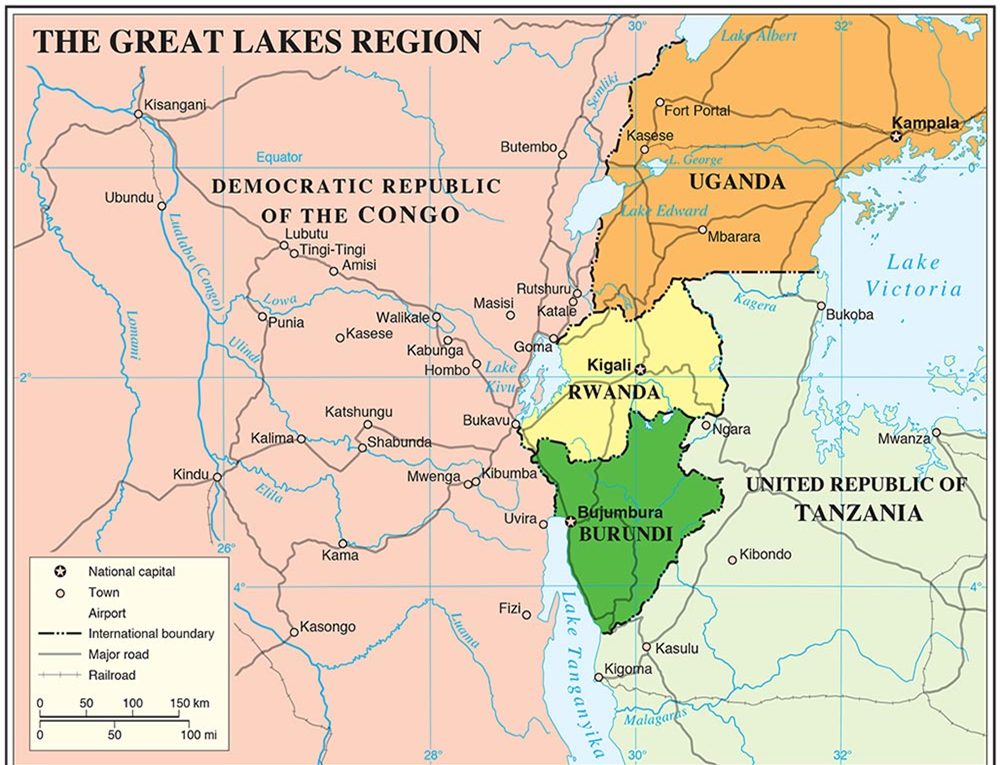
\includegraphics[scale=0.40]{pictures/week24.png} 
\end{frame}

\frame{
\frametitle{Conclusion}
\begin{center}
All clear? More questions? \\
See you next week!
\end{center}
}

\end{document}